\subsubsection{Airy function}

First, we define the function we call Airy. 
$$Ai(x) \deff \frac{1}{2\pi \ii} \int_{\Gamma} \ee^{-\frac{1}{3} z^3 + x z} \dd z$$ 
Let's take $\Gamma$ to be the union of the two half open line $\Gamma = (\ee^{-2\pi\ii / 3}\infty, 0] \cup [0, \ee^{2\pi\ii / 3} \infty)$. Of course, by Cauchy Theorem, we know that the definition is independent of the contour as long as the contour goeas from $\ee^{-2\pi\ii / 3}\infty$ to $\ee^{2\pi\ii / 3}\infty$. Now, we need to get things in order to apply Laplace method on the integral. We could start defining
$$g(z) = \ee^{-\frac{1}{3} z^3}, \ \ f(z) = z$$
but this is not a good approach as such an $f$ won't have any critical points and won't help us calculate the integral. We then try a change of variable to get a function with those critical points. Define $x \deff \lambda \ee^{\ii \theta} = \lambda \omega$ so that we can send $x$ to infinite by sending $\lambda$ in a constant direction $\theta$. Now, introduce a variable $s$ such that $s\lambda^{\eta} = z$ for some $\eta \in \R$. Now, we want to extract $\lambda$ from the new exponent 
$$-\frac{1}{3}\lambda^{3\eta}s^3 + \lambda^{1+\eta} \omega s$$
so we set $\eta = 1/2$ and have that
$$Ai(\lambda, \theta) = \frac{\lambda^{\frac{1}{2}}}{2\pi \ii} \int_{\Gamma} \ee^{-\lambda^{\frac{3}{2}}(s^3/3 - \omega s)} \dd s$$
$$\implies Ai(\lambda, \theta) = \frac{\lambda^{\frac{1}{2}}}{2\pi \ii}\Phi(\lambda^{\frac{3}{2}}) , \ \ \Phi(\lambda) = \int_{\Gamma} \ee^{-\lambda f(s)} \dd s, \ \ f(s) = f_{\omega} \deff \frac{s^3}{3} - \omega s $$ 
Note that we have $f$ with two critical points, $s_c^{\pm} = \pm \sqrt{\omega}$. We now need to study the steepest descent path. For reasons that will be clear soon, we divide the analysis into the cases
\begin{enumerate}
	\item $\theta = 0$
	\item $0< \theta < \frac{2}{3} \pi$	
	\item $\theta = \frac{2}{3} \pi$
	\item $\frac{2}{3} \pi < \theta < \pi$
	\item $\theta  = \pi$
\end{enumerate}
the rest of the cases should follow from the same arguments based on the symmetry of the critical points. For each case we want to deform $\Gamma$ to a new contour $\tilde{\Gamma}$ such that
\begin{description}
	\item[(a)] $\tilde{\Gamma}$ is homotopically equivalent to $\Gamma$, in the sense that the integral in the definition of $\Phi(\lambda)$ is invariant under the deformation from $\Gamma$ to $\tilde{\Gamma}$.
	\item[(b)] The contour $\tilde{\Gamma}$ is a level line of $\Im{(f)}$ that passes through one of the critical points of $f$.
\end{description}

For $(a)$ to be true we need to guarantee that the deformed path $\tilde{\Gamma}$ should start at $\infty \ee^{-\ii \theta}$ and end at $\infty \ee^{\ii \theta}$ for some $\theta \in [\pi/2, 5\pi/6]$. Now we need to discuss how to satisfy $(b)$ for every one of the cases cited. For all cases, we refer to Image \ref{Fig: theta cases} for illustration of the scenario and intuition on the contour lines we take.

For the first case, $(1)$, we  ca see that the integration path can be taken as the union of the lines emerging from $s_c^-$ with angle $\pi/2$ and $3\pi/2$. For the second case we note that something happens when $\theta = 2/3 \pi$. This is because $f(s_c^+) = f(s_c^-)$ when $\theta = 2/3 \pi$. But until this point the topology is equivalent. For this interval of values then we take the path of integration to be basically the same as before, the union of the lines emerging from $s_c^-$ with angle $\pi/2$ and $3\pi/2$.

For both of these cases we have the integration of $\Gamma$ to be given by the contribution of the critical point $s_c^-$ by the asymptotic of Laplace.

For $\theta = 2/3 \pi$, case $(3)$, something change. We now need to take a path that passes through both critical points. WE would think that now we have to consider the asymptotic from both saddle points but, in reality, because $Re(f(s_c^-)) < Re(f(s_c^+))$ the contribution from $s_c^-$ exponentially dominates the asymptotic.

For case $(4)$ we no longer have a clear connection of the lines. We need to take $\tilde{\Gamma}$ to be the union of two disjoint curves: The line coming from $\infty \ee^{-\ii 2\pi/3}$ passing through $s_c^-$ and going to infinity parallel to the real line and the line coming from infinity parallel to the real line, passing through $s_c^+$ and going to $\infty \ee^{\ii 2\pi/3}$. Again,  the contribution from $s_c^-$ exponentially dominates the asymptotic.

For case (5), when $\theta = \pi$, the path of steepest descent is similar to the one just taken. But a key difference is to be noted, now, as $Re(f(s_c^-)) = Re(f(s_c^+))$, contributions from both saddle points must be accounted in the asymptotic.


\begin{figure}[h] 
	\centering
	\subfigure{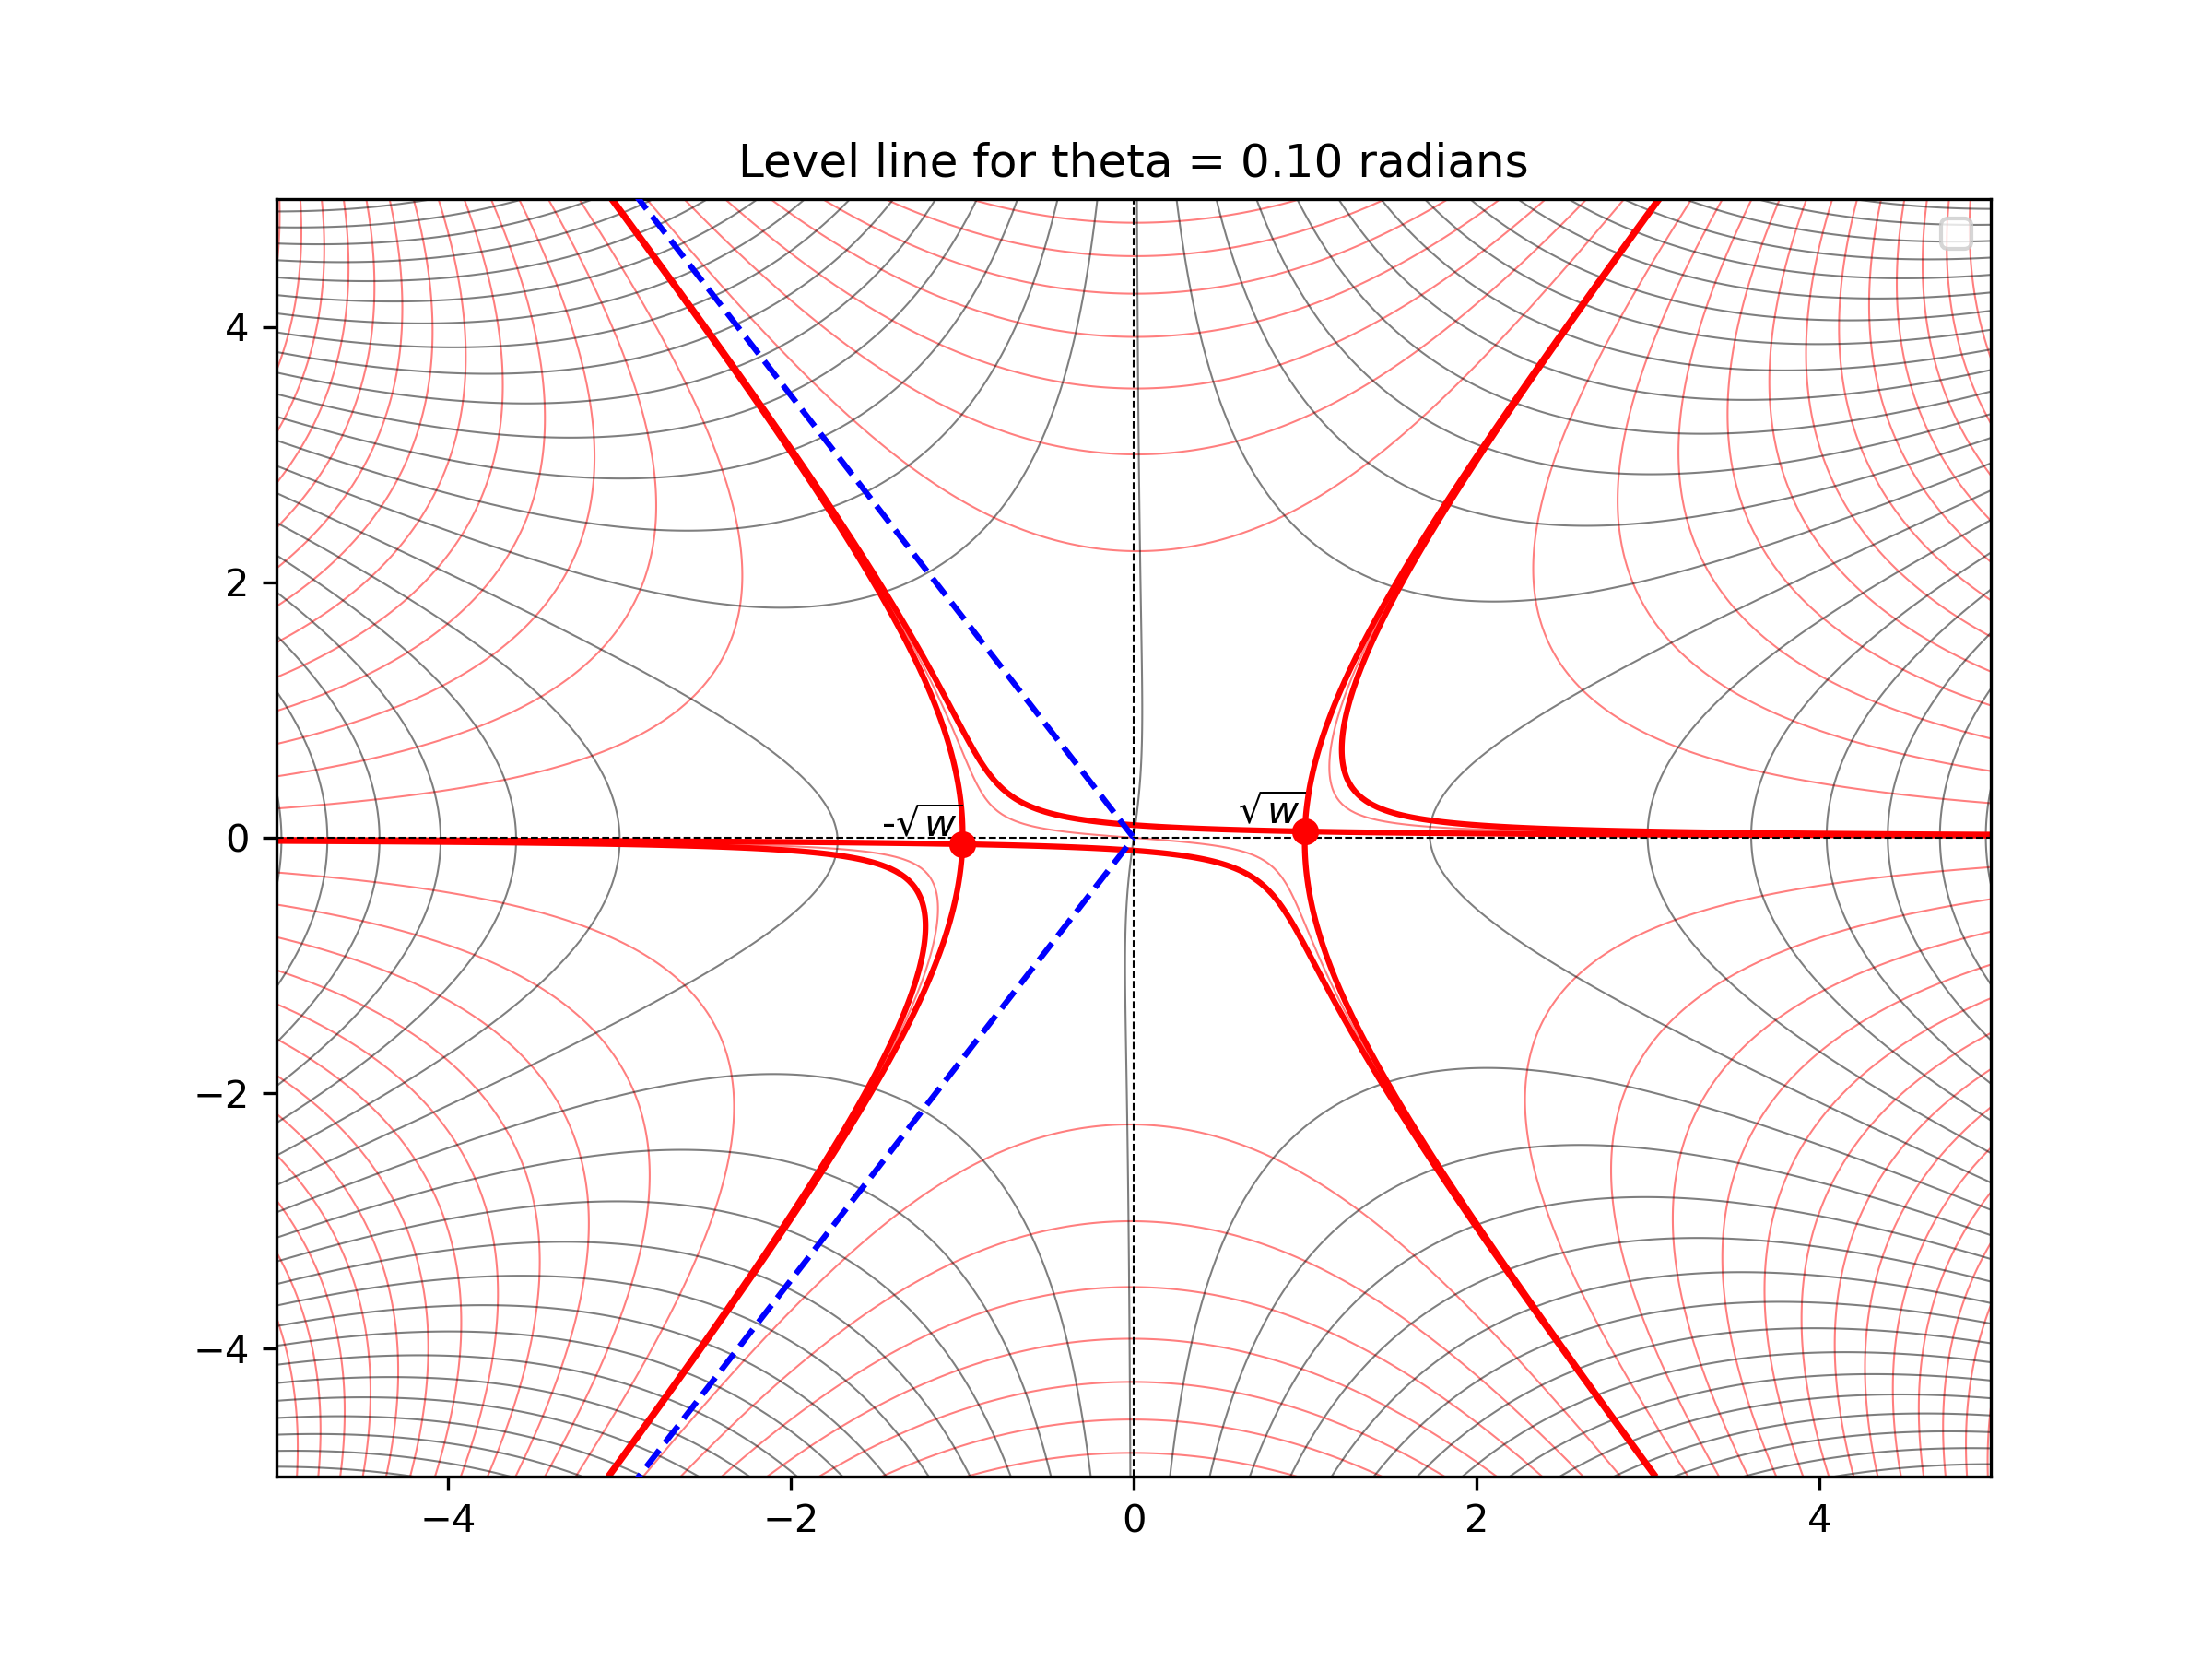
\includegraphics[width=0.49\textwidth]{/home/vap/Documents/RMT-TEX/NotasMsC/Assets/contour_plot_theta_0.10.png}}
	\subfigure{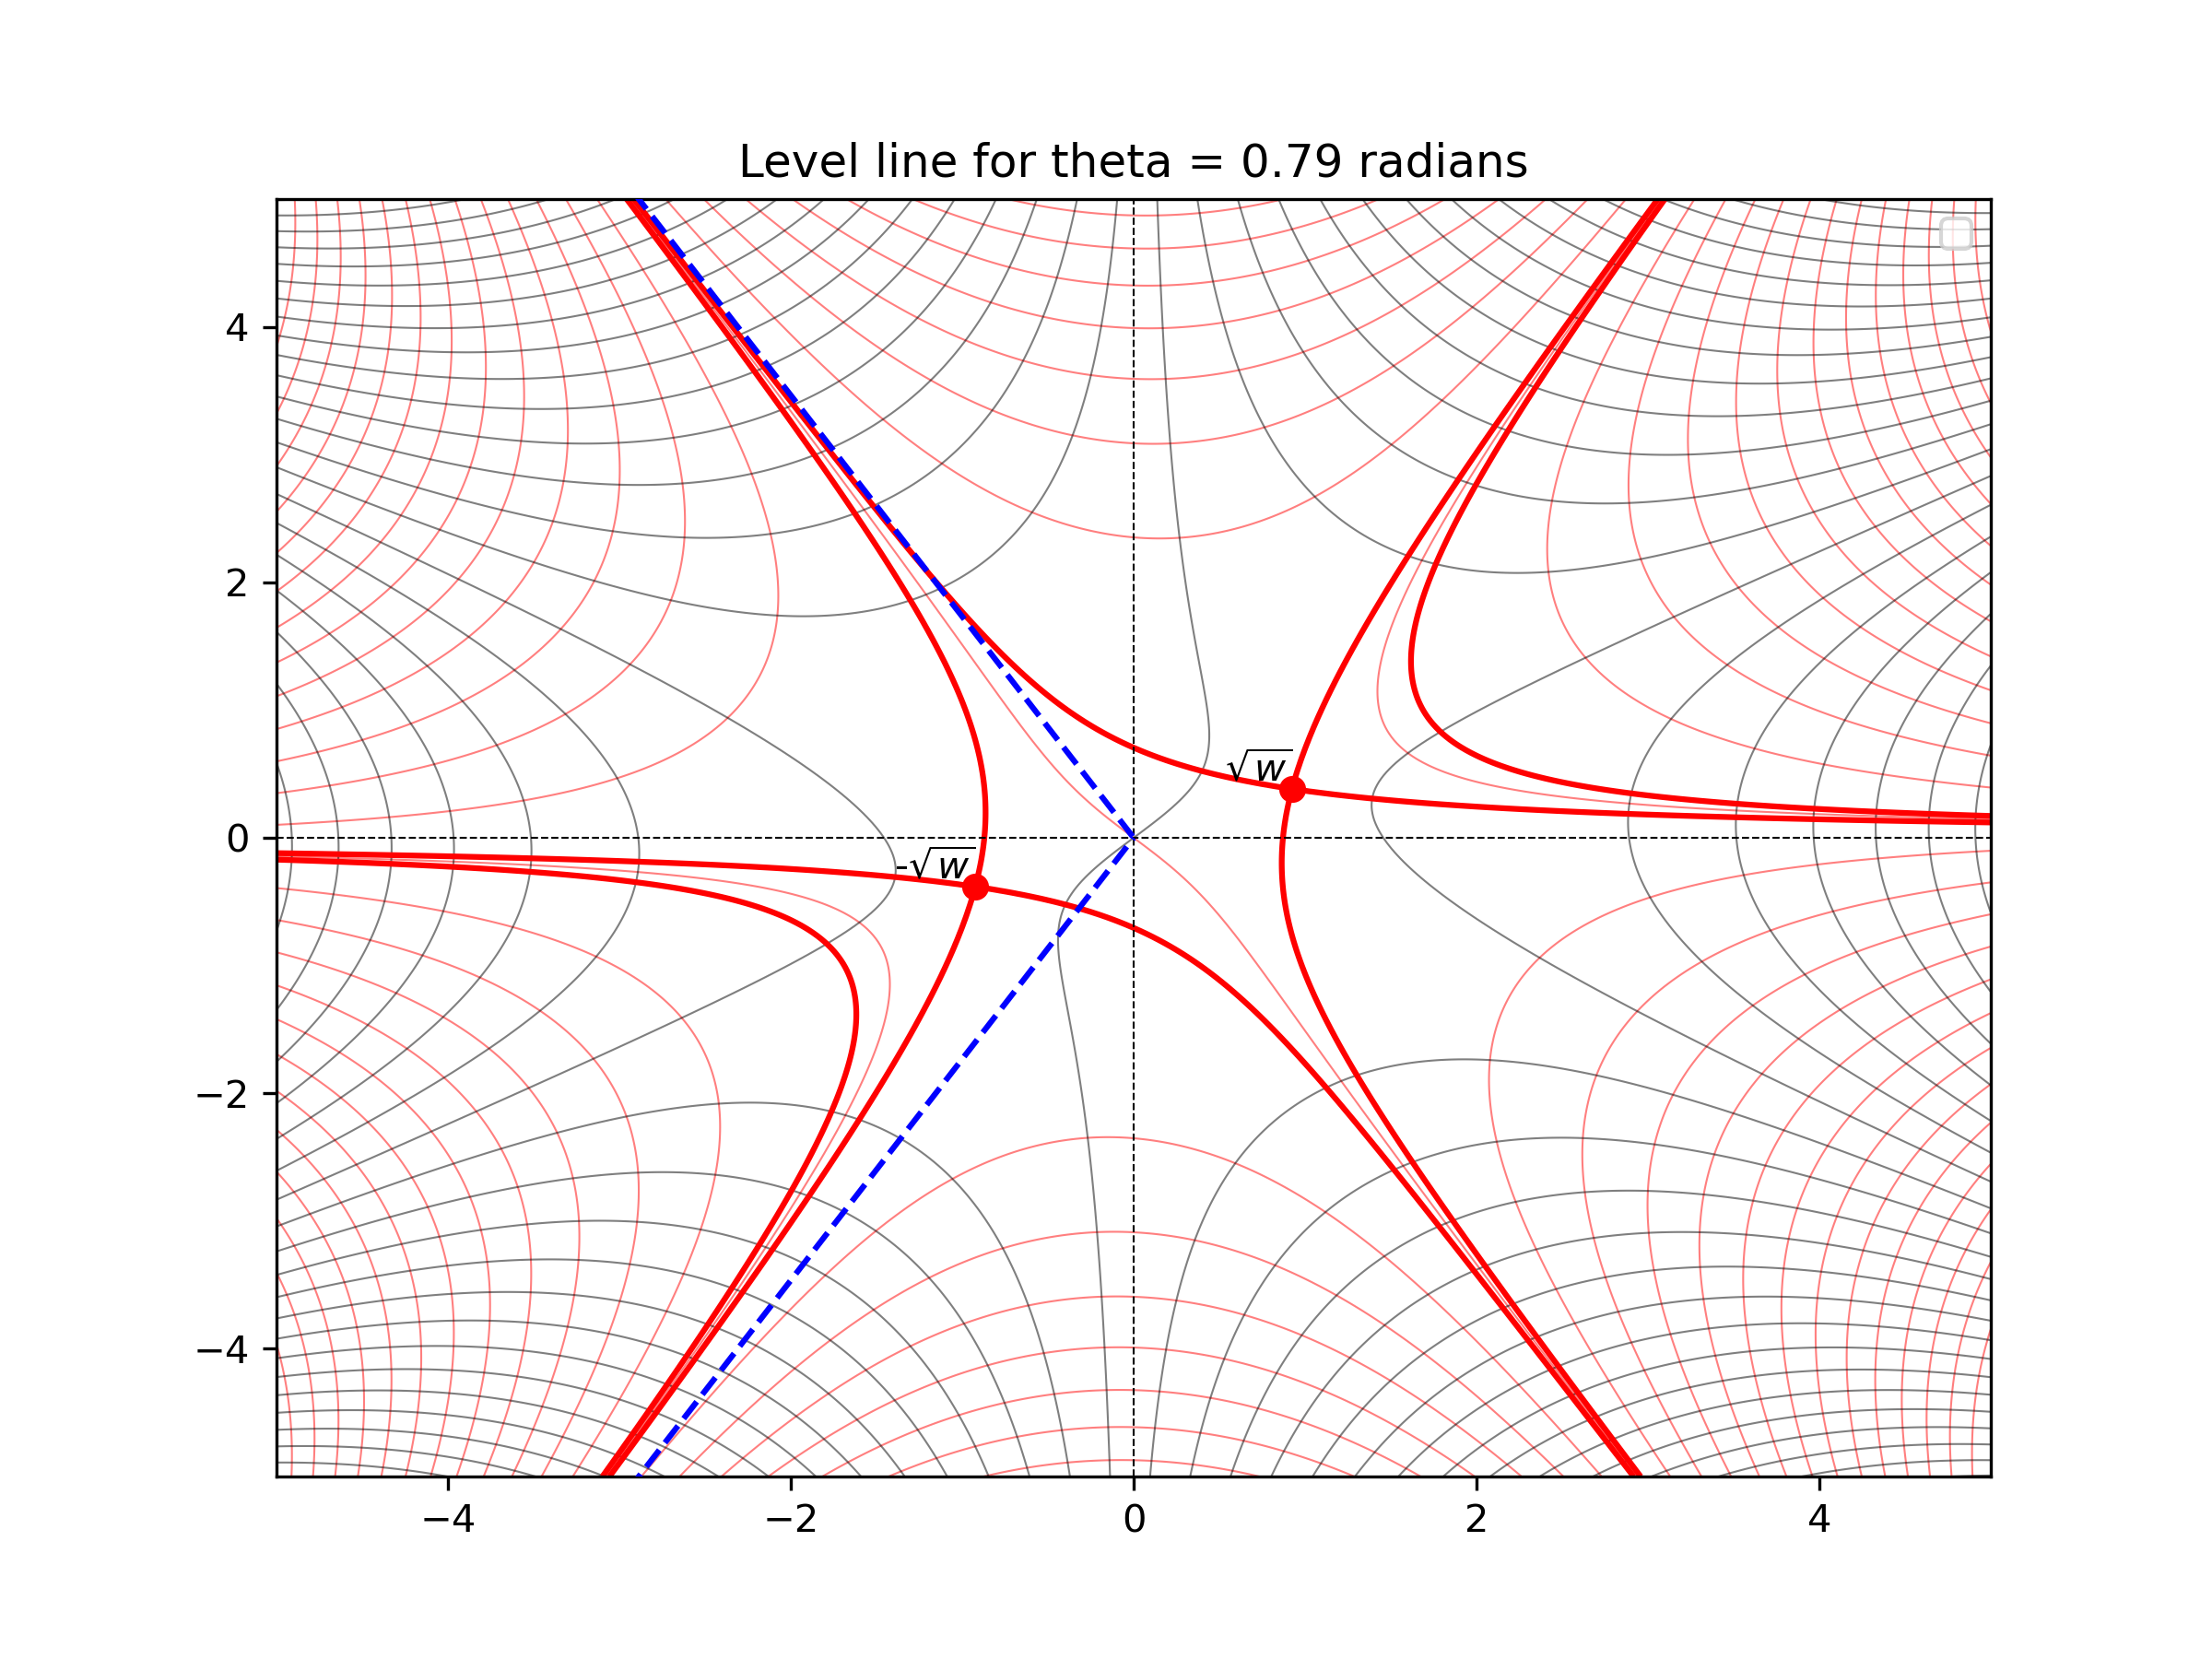
\includegraphics[width=0.49\textwidth]{/home/vap/Documents/RMT-TEX/NotasMsC/Assets/contour_plot_theta_0.79.png}}
	\subfigure{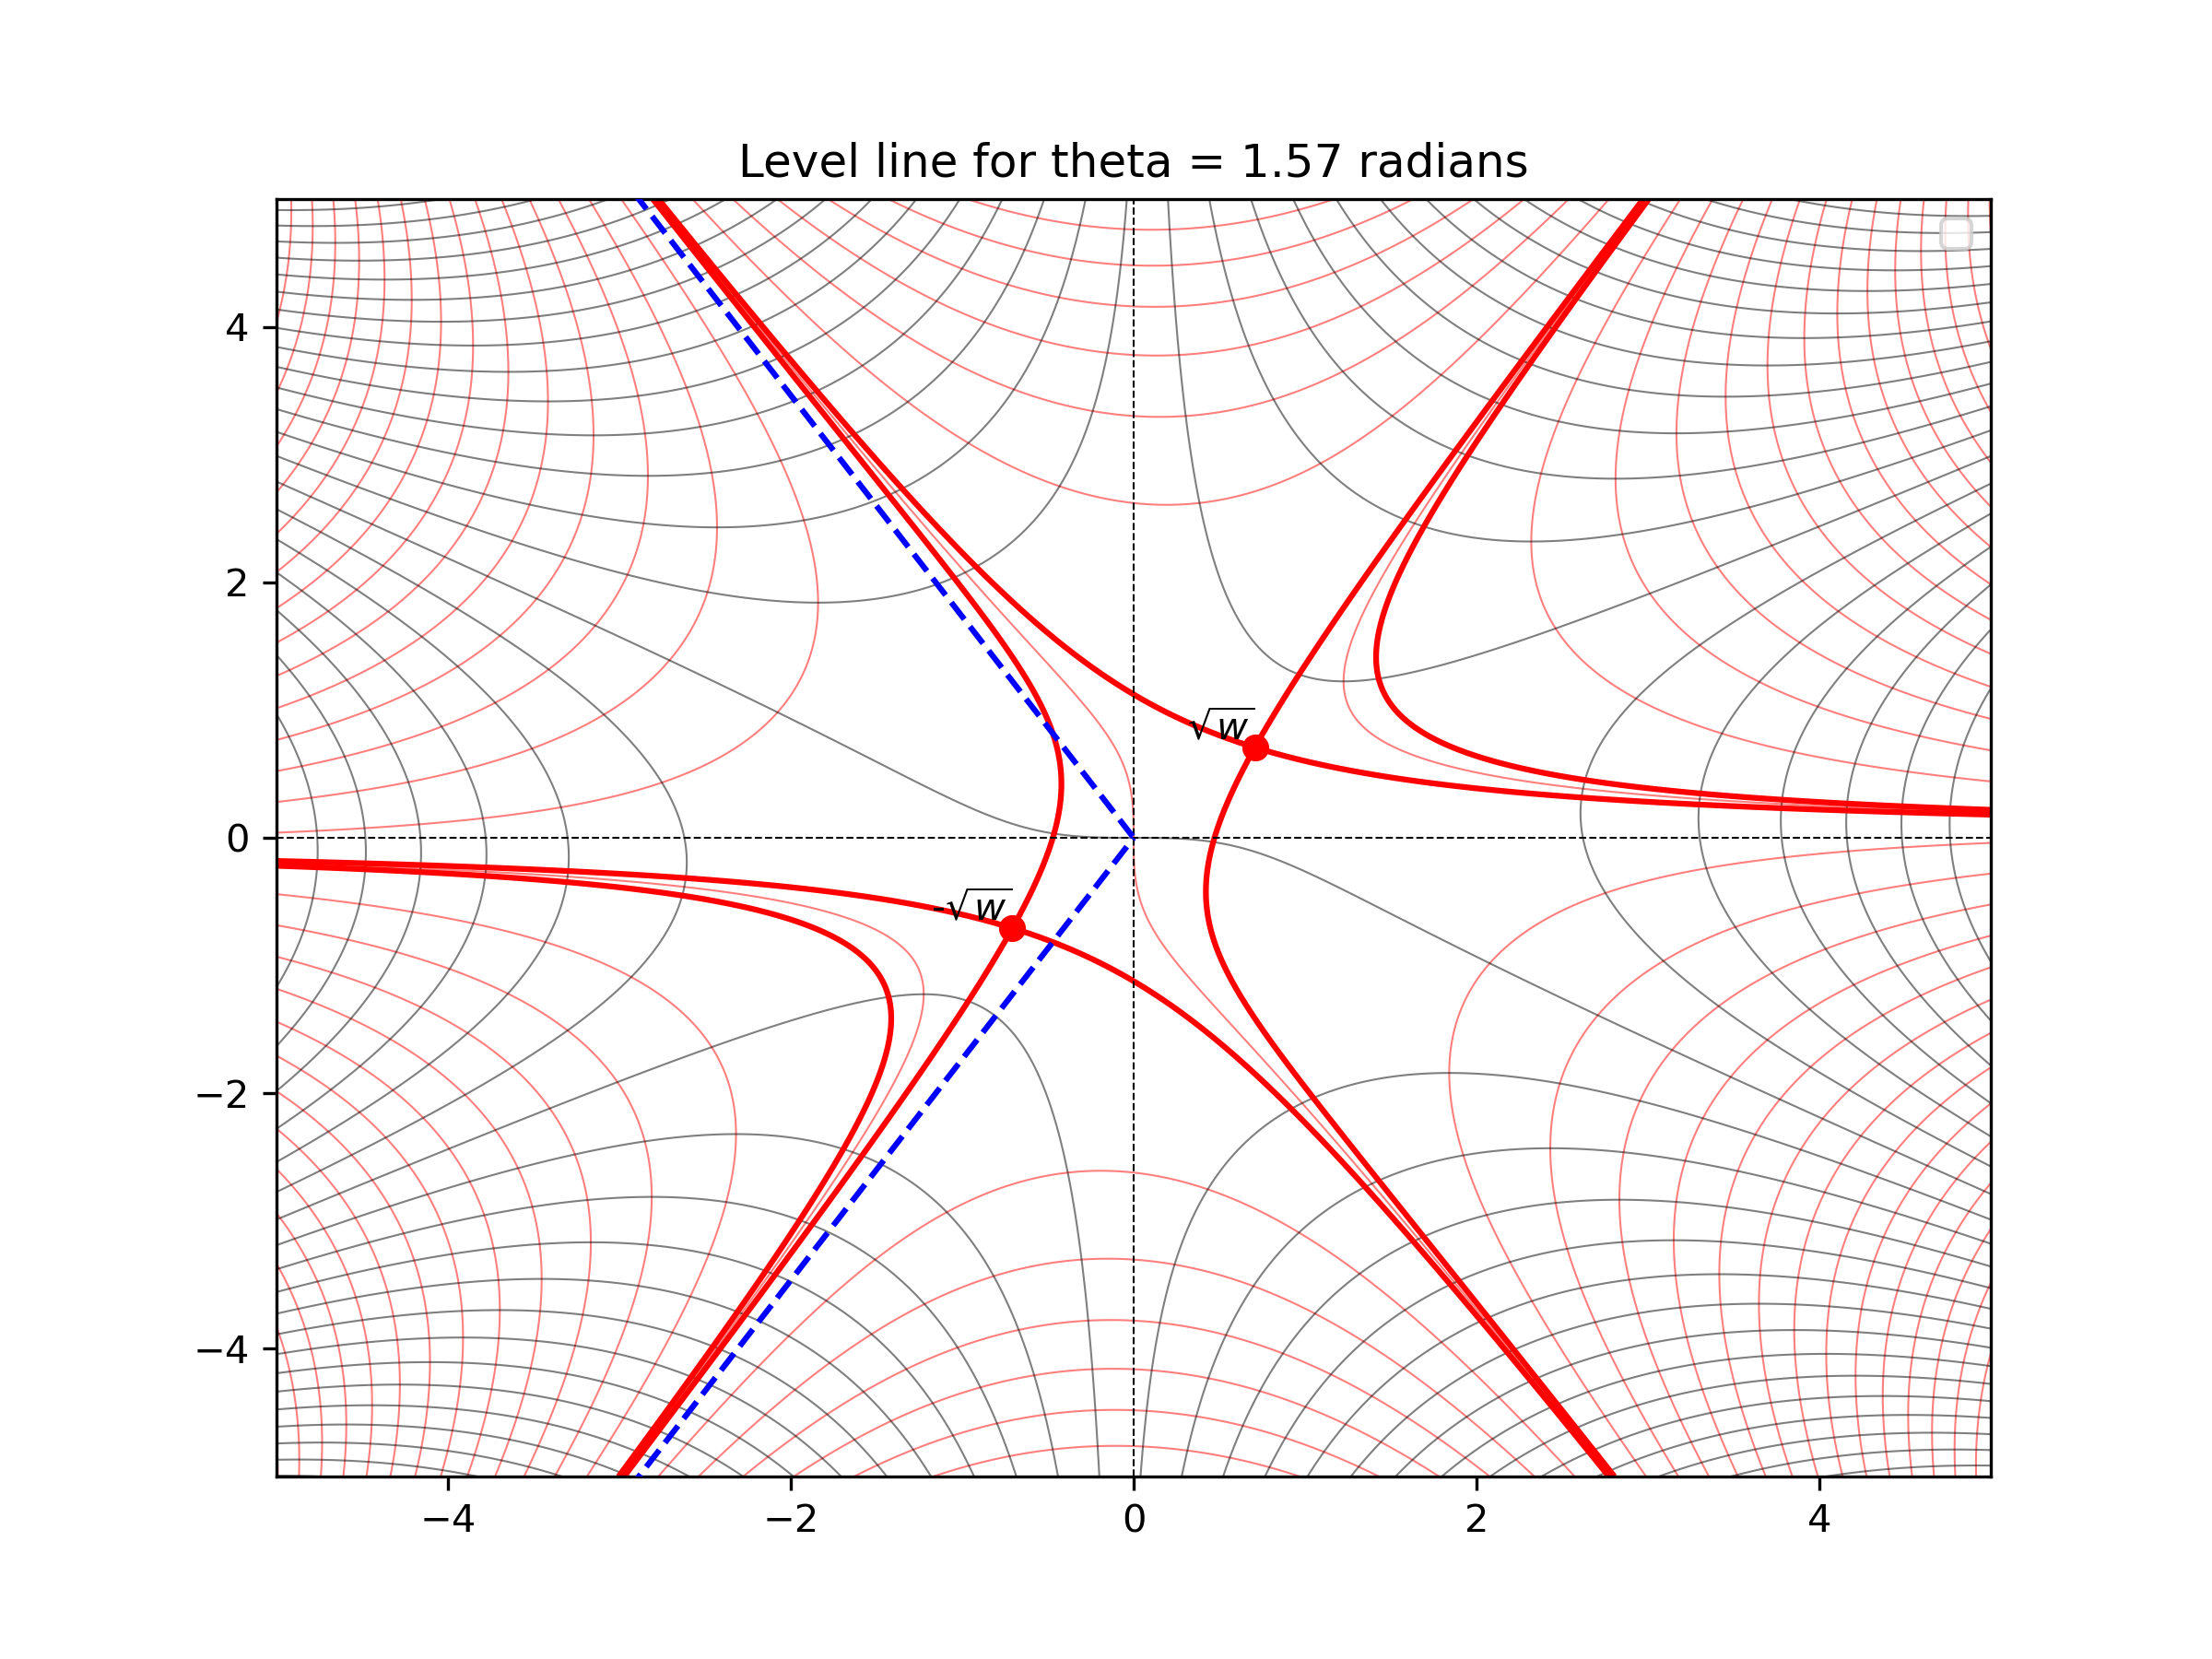
\includegraphics[width=0.49\textwidth]{/home/vap/Documents/RMT-TEX/NotasMsC/Assets/contour_plot_theta_1.57.png}}
	\subfigure{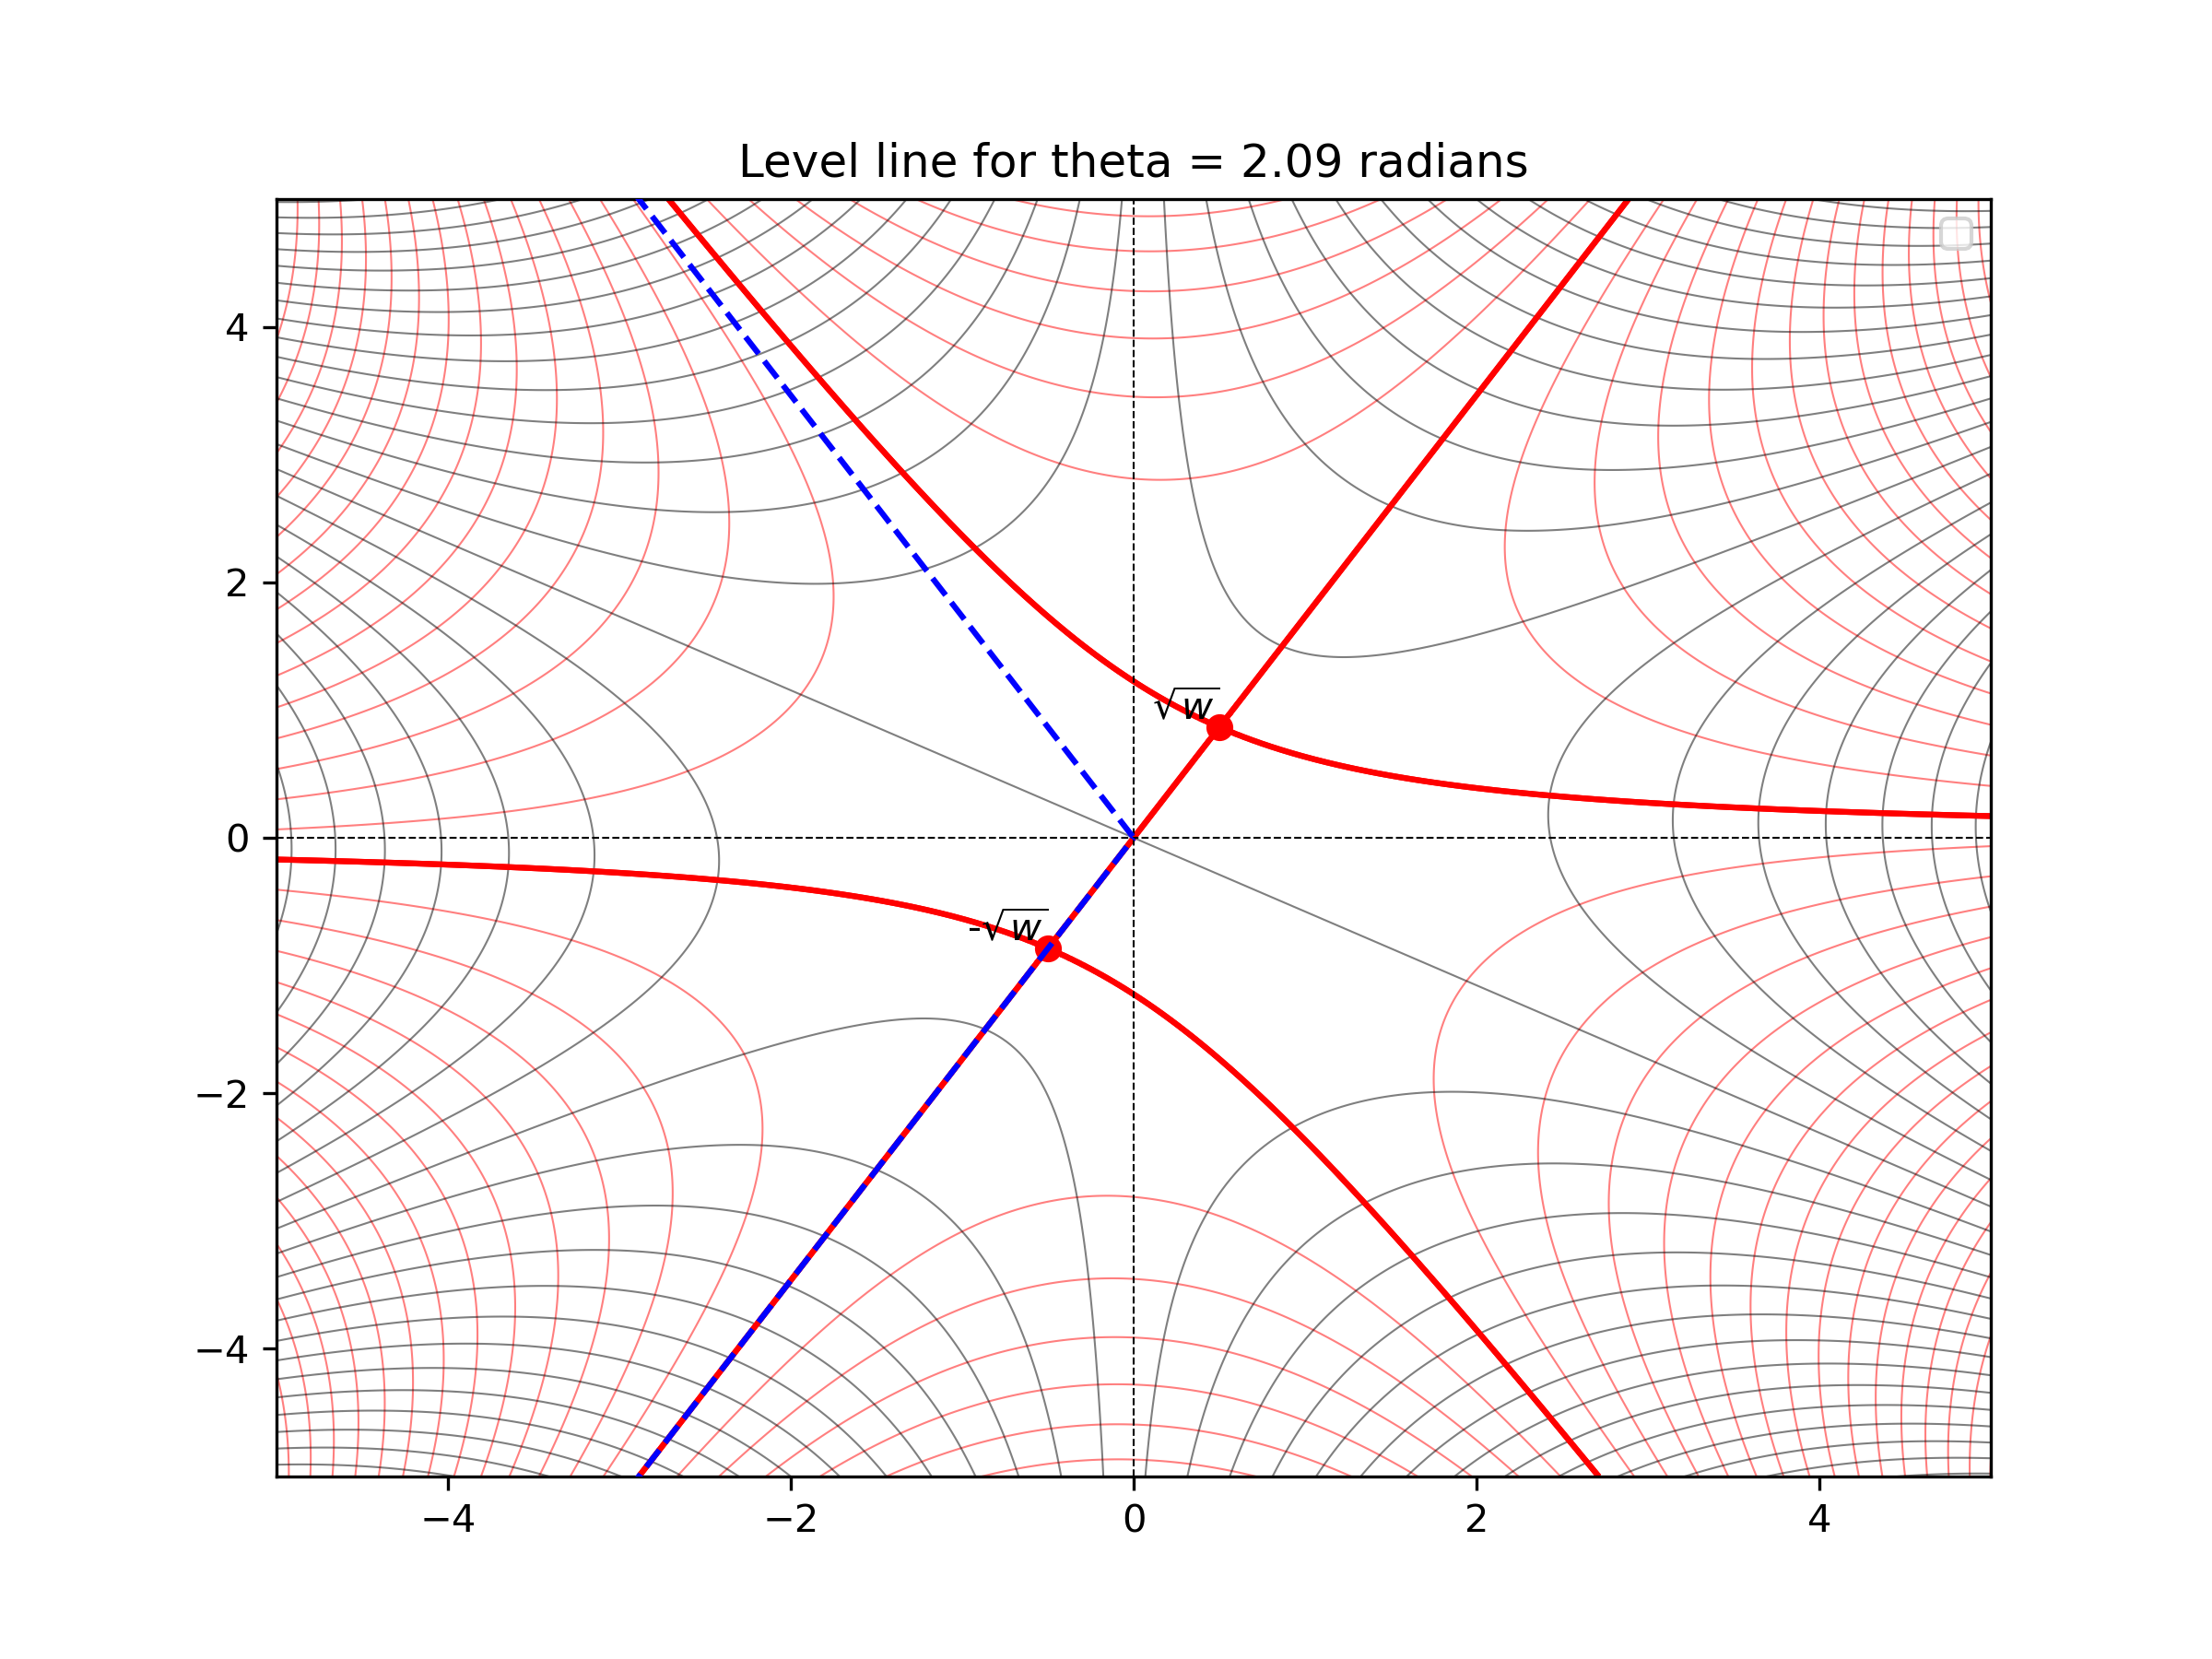
\includegraphics[width=0.49\textwidth]{/home/vap/Documents/RMT-TEX/NotasMsC/Assets/contour_plot_theta_2.09.png}}
	\subfigure{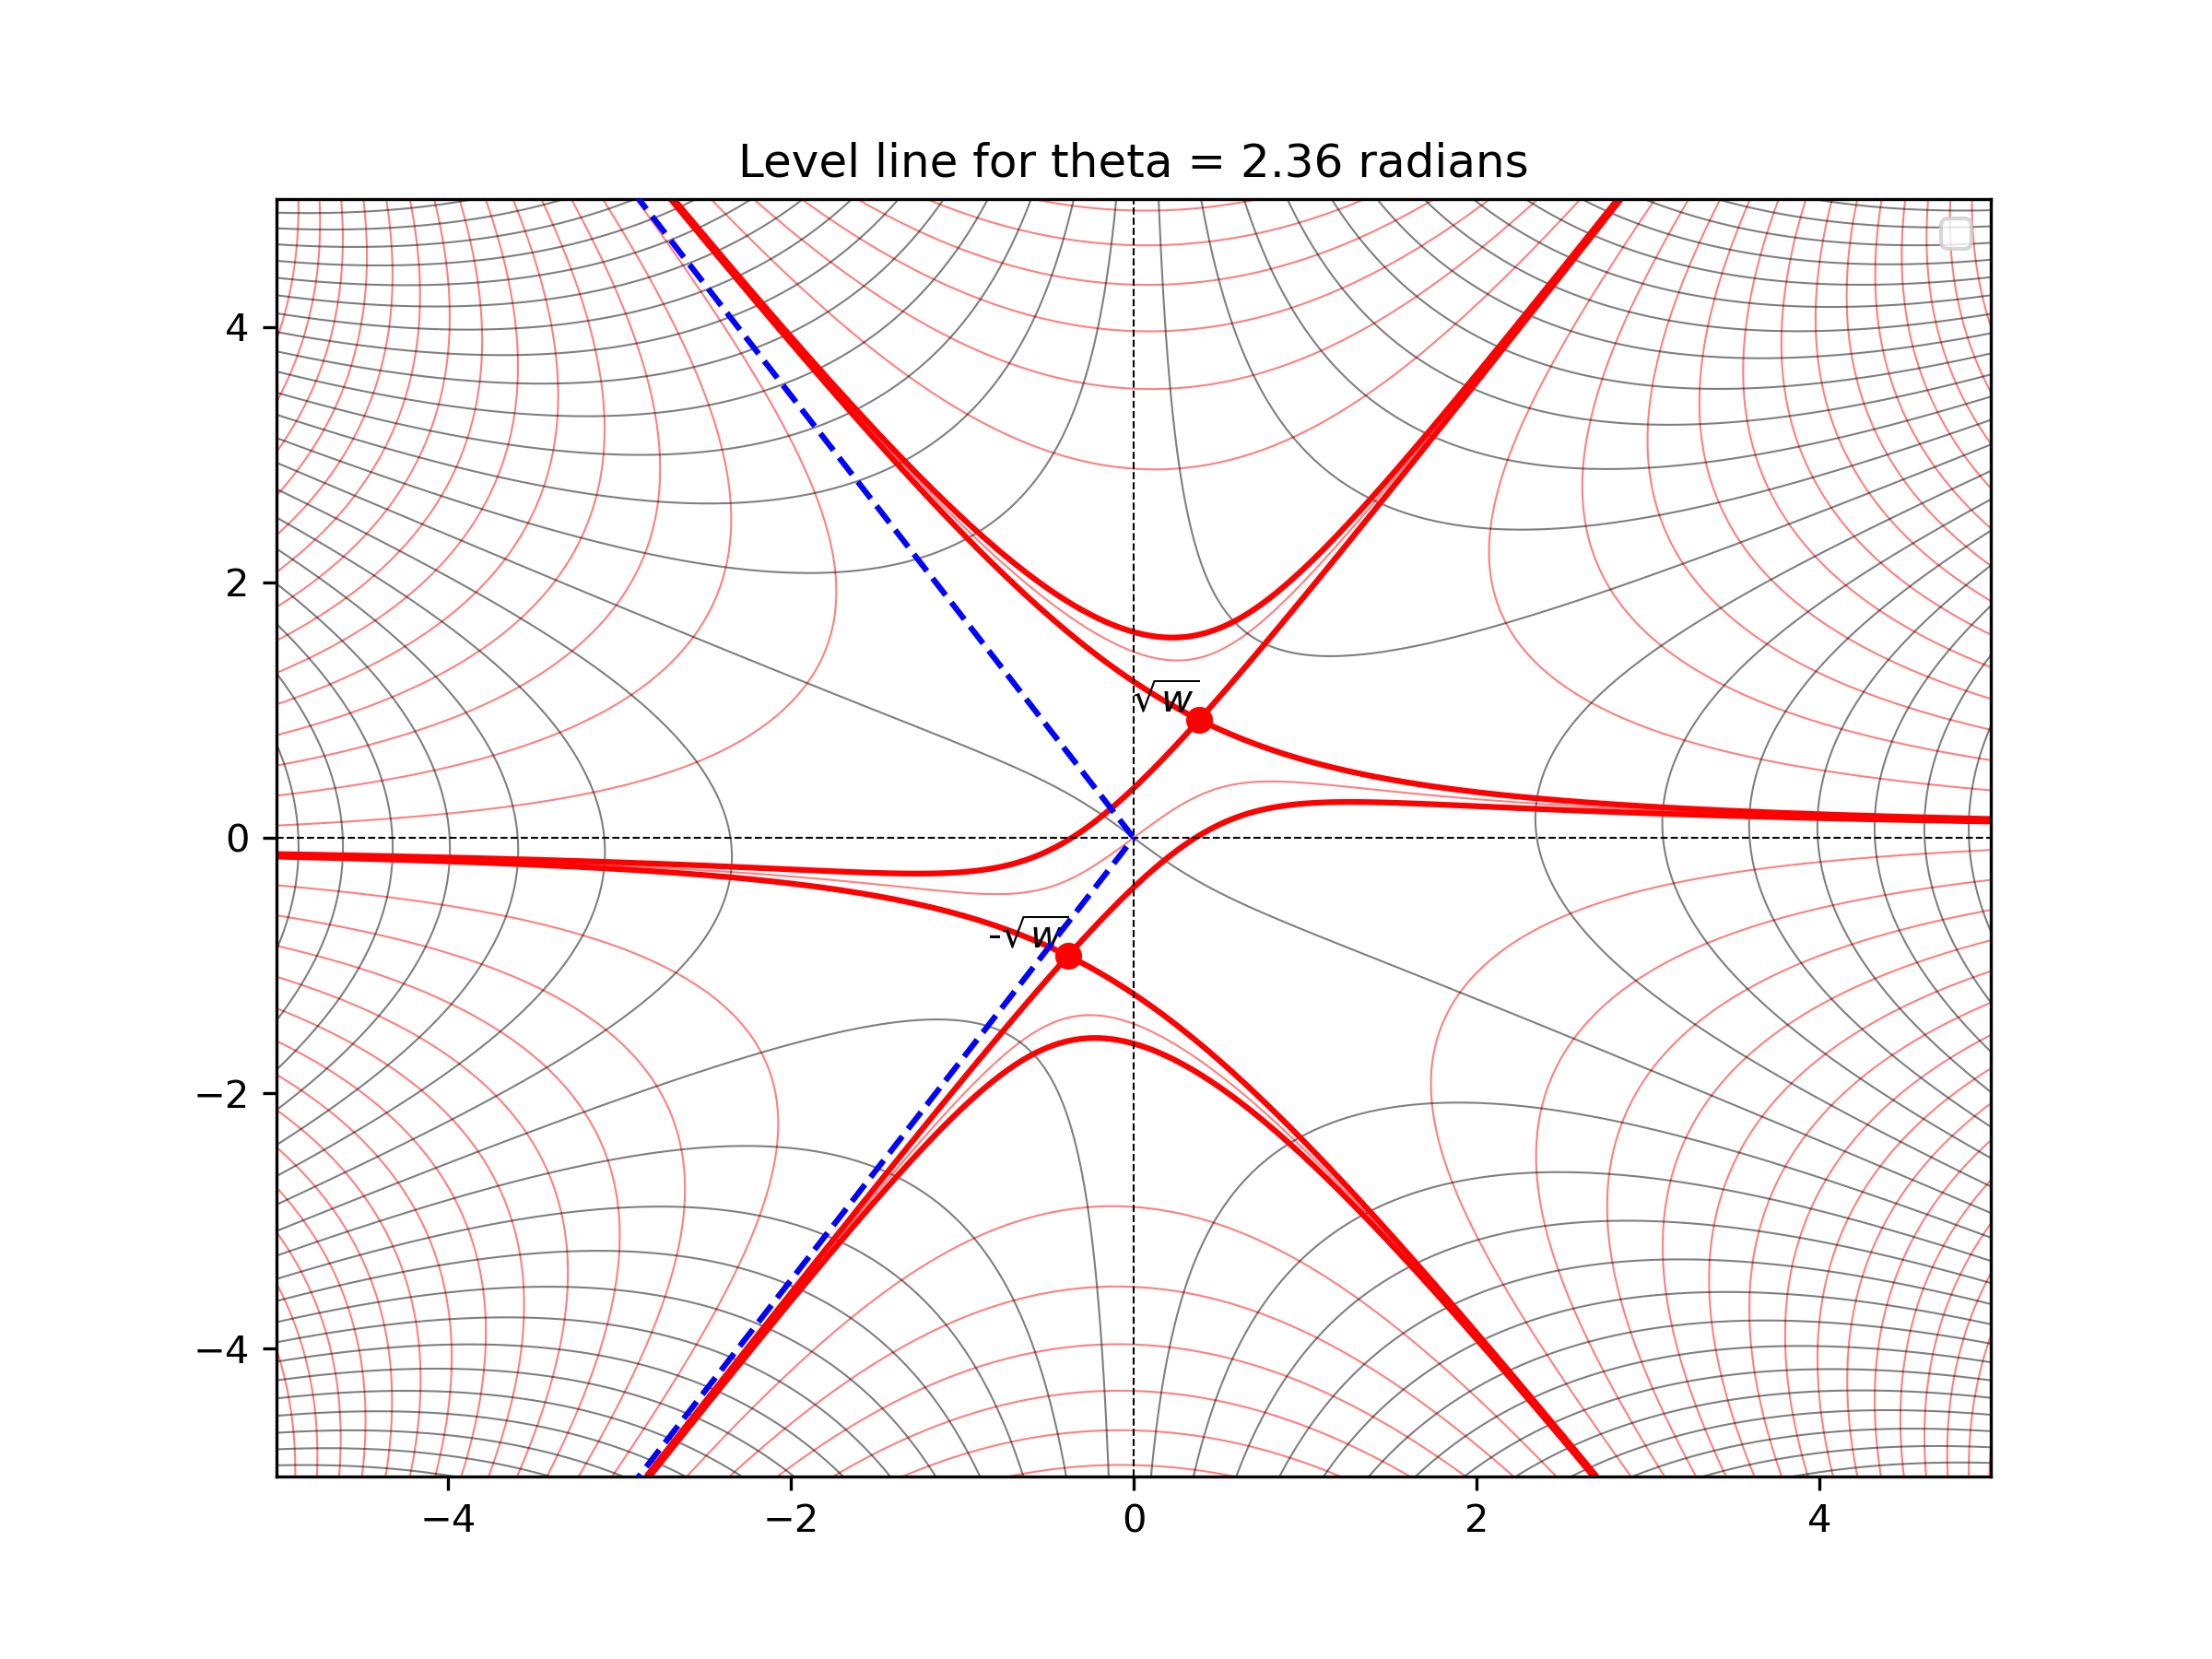
\includegraphics[width=0.49\textwidth]{/home/vap/Documents/RMT-TEX/NotasMsC/Assets/contour_plot_theta_2.36.png}}
	\subfigure{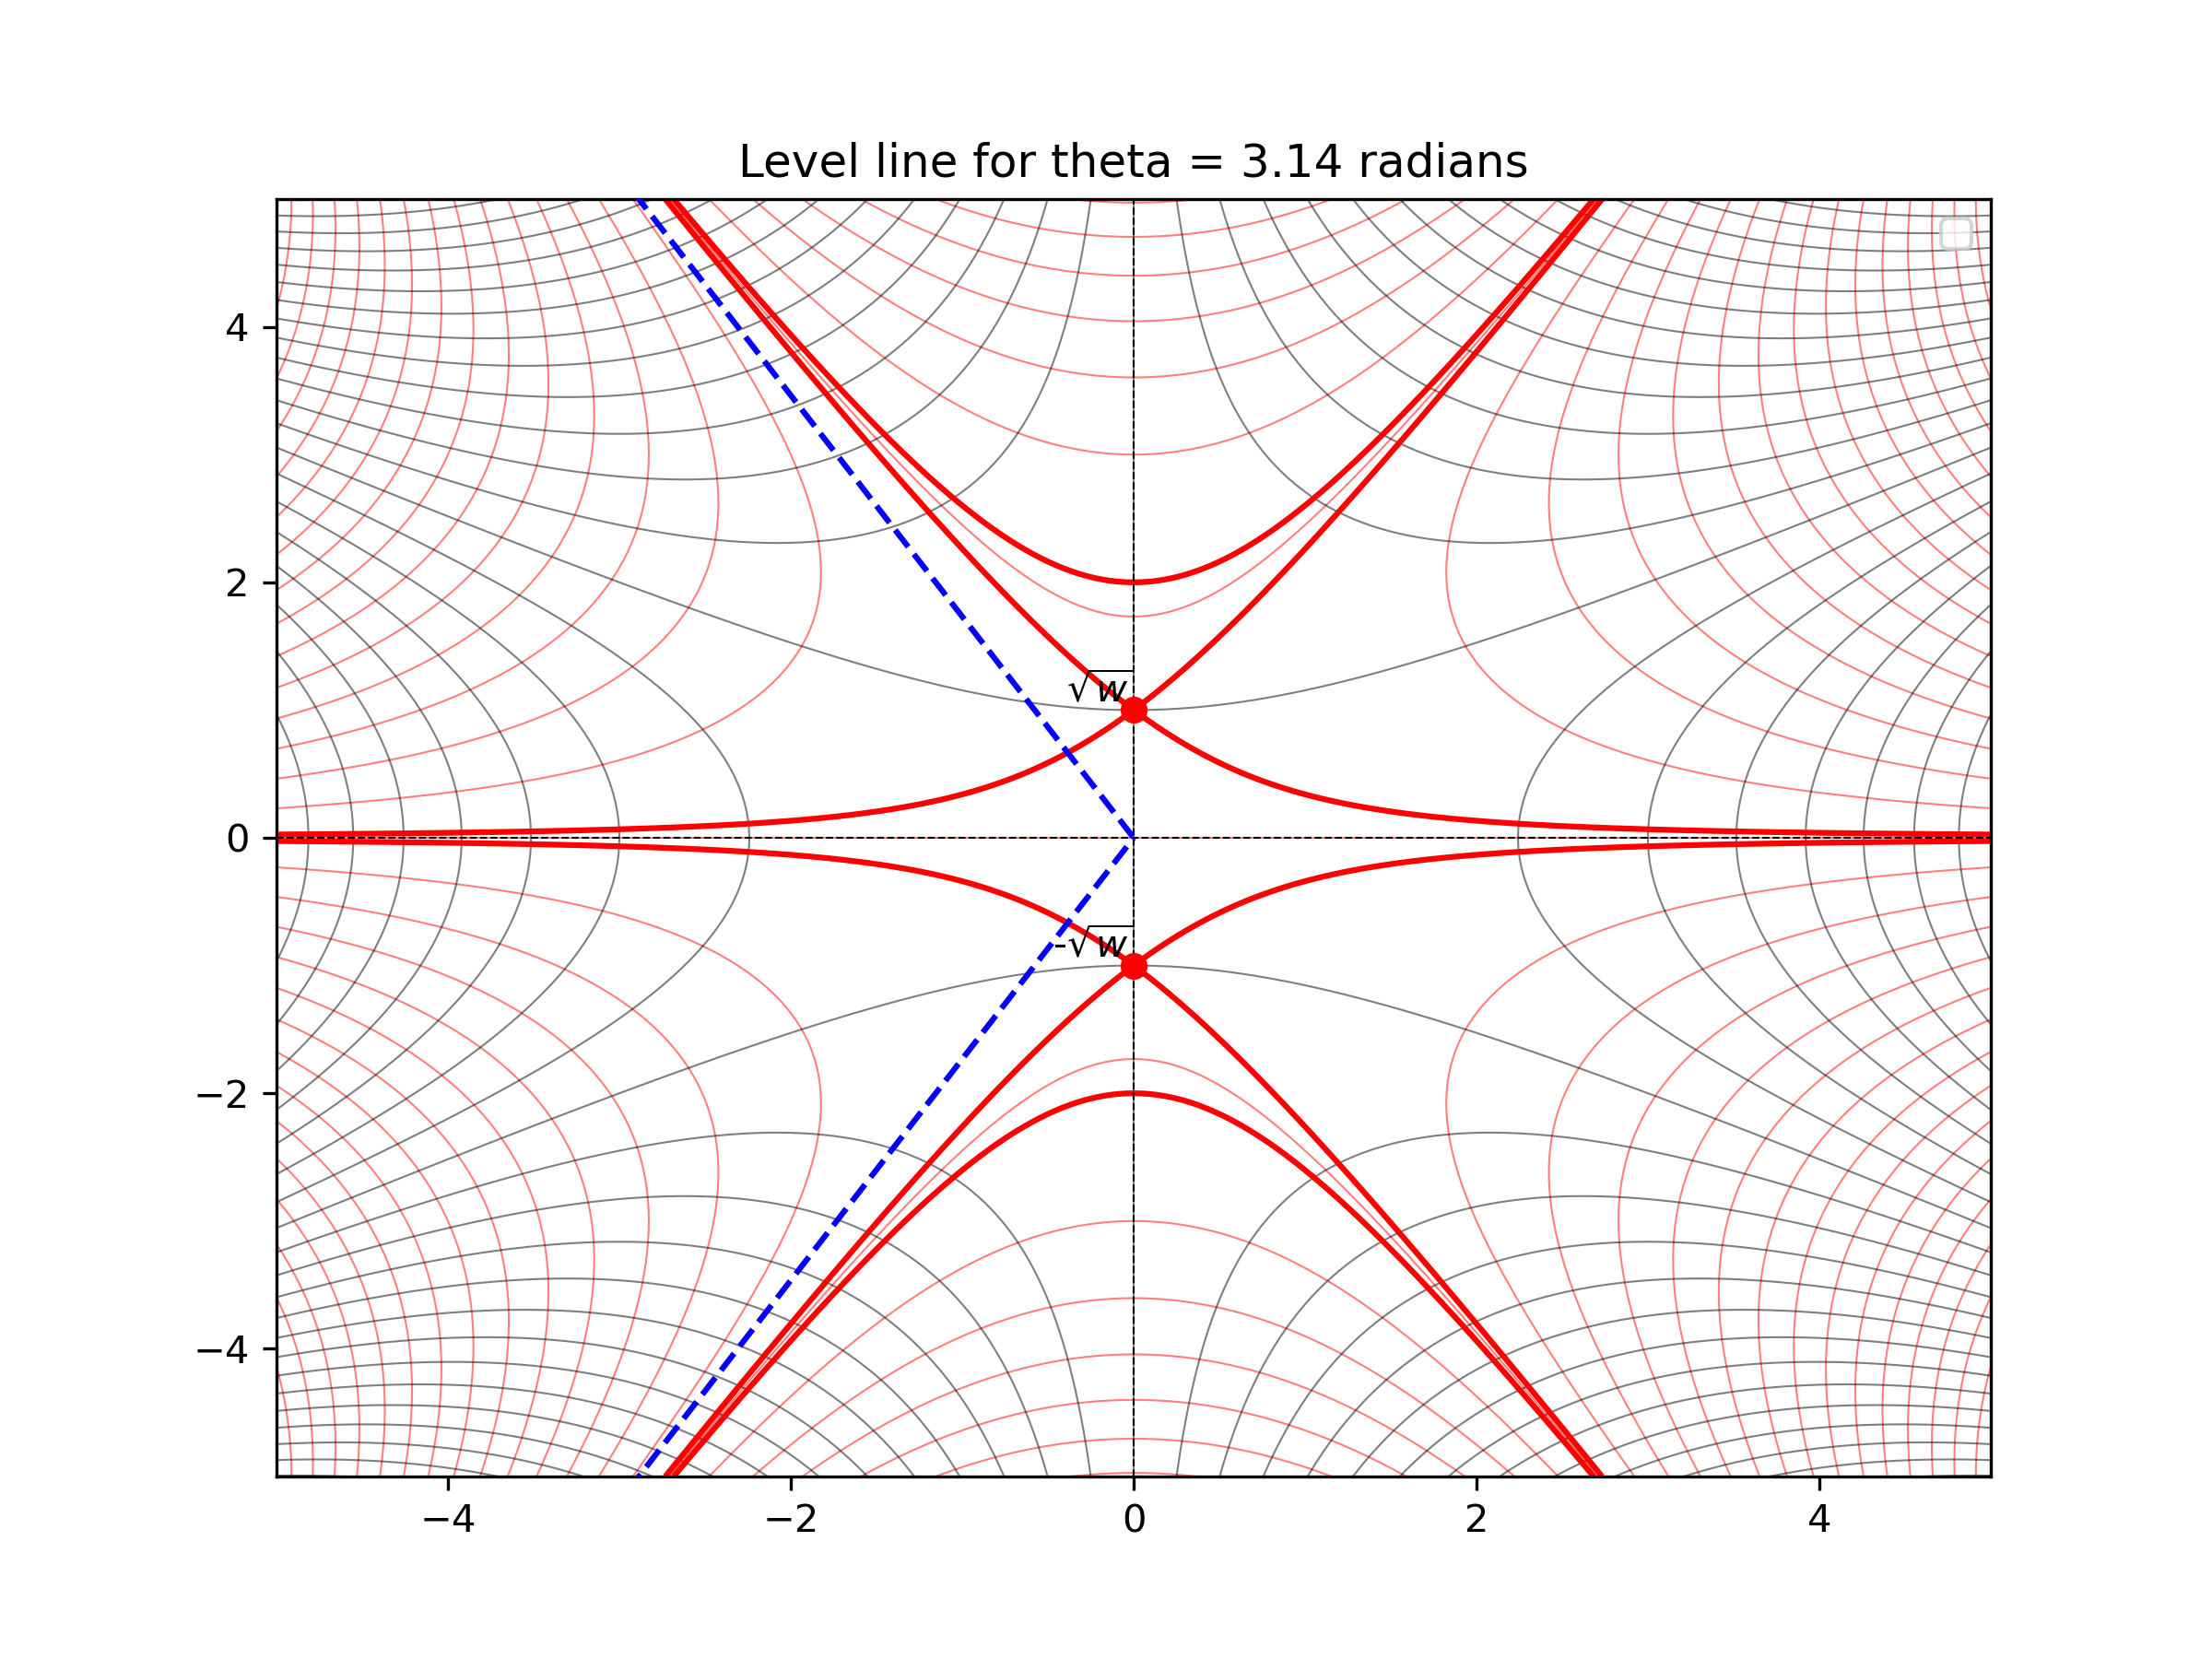
\includegraphics[width=0.49\textwidth]{/home/vap/Documents/RMT-TEX/NotasMsC/Assets/contour_plot_theta_3.14.png}}
	\caption{Scenarios for $\theta$}
	\label{Fig: theta cases}
\end{figure}